\section{Cota inferior del anti-thickness geométrico de $K_n$}\label{sec:cota_inf}
El principal resultado de este trabajo es que encontramos el valor exacto del
anti-thickness geométrico para la gráfica completa con hasta diez vértices en
posición general. Obtuvimos dicho valor mejorando la cota inferior y usando la cota superior actual, las cuales siguen a continuación:
\begin{equation}
\left\lfloor\frac{n-1}{2}\right\rfloor \leq At_g(K_n) \leq n - \left\lfloor
\sqrt{2n + \frac{1}{4}} - \frac{1}{2} \right\rfloor.
\label{ecuacion_cotas_atg}
\end{equation}

De manera general, si se desea encontrar una cota superior para el
anti-thickness geométrico de $K_n$ es necesario encontrar una descomposición en
thrackles, para cualquier dibujo de $K_n$. La cota superior trivial del
anti-thickness geométrico de $K_n$ es $\binom{n}{2}$ ya que cada arista de
$K_n$ es un thrackle. Si se desea encontrar una cota inferior es necesario
demostrar, para todo dibujo de $K_n$, cuántos thrackles son necesarios para dar
una descomposición en thrackles.

Empezamos explicando la cota inferior conocida para el anti-thickness
geométrico y después diremos cómo la mejoramos para $n\leq 10$.

Un conjunto de $n$ puntos en el plano induce una gráfica completa con $n$
vértices a la que denotamos como $K_n$. Como es completa $|E(K_n)|=
\binom{n}{2}$.
Cuando se quiere encontrar una descomposición de tamaño mínimo en thrackles una
idea que resulta intuitiva es buscar que los thrackles tengan el mayor número
posible de aristas. El siguiente teorema es útil para nosotros ya que establece
el número máximo de aristas que puede tener un thrackle geométrico.
\begin{theorem}(\cite{Pach2013b})
  Toda gráfica geométrica de $n$ vértices en la
  que no existen dos aristas disjuntas tiene a lo más $n$ aristas. Esto se
  cumple para toda $n>2$.
\end{theorem}

Omitimos la demostración del teorema anterior ya que las ideas de la
demostración no son retomadas en este trabajo.
% El teorema es importante para
% nosotros ya que indica el número máximo de aristas posibles para un thrackle.

Como mencionamos en el capítulo de antecedentes, un thrackle de $n$ vértices
con exactamente $n$ aristas es un thrackle máximo. Por definición, toda
descomposición de la gráfica completa cubre sus aristas. Si suponemos que
existen $k$ thrackles máximos en la descomposición, entonces la siguiente
desigualdad expresa el número de thrackles máximos necesarios para cubrir las
$\binom{n}{2}$ aristas de la gráfica completa:
\[ kn \geq \binom{n}{2}. \]

Como los thrackles de la descomposición son geométricos, si buscamos la $k$ más
pequeña para la cual se cumple la desigualdad anterior entonces $k$
sería el anti-thickness geométrico de la gráfica completa.
Resolviendo para $k$  tenemos que al menos
$k\geq\left\lceil\frac{n-1}{2}\right\rceil$ thrackles máximos son necesarios
para dar una descomposición de $K_n$. En otras palabras
\begin{equation}
  At_g(K_n) \geq  \left\lceil\frac{n-1}{2}\right\rceil.
  \label{resultados_cotainf_1}
\end{equation}

La tabla~\ref{table:attrivialinf} ilustra el valor de la cota inferior del
anti-thickness geométrico dada por la desigualdad \ref{resultados_cotainf_1}
para $n\leq 10$.
\begin{table}[t]
  \centering
  \begin{tabular}{|c|c|}
    \hline
    $n$ & $\left\lceil\frac{n-1}{2}\right\rceil$ \\[5pt] \hline\hline
    3   & 1  \\
    4   & 2  \\
    5   & 2  \\
    6   & 3  \\
    7   & 3  \\
    8   & 4  \\
    9   & 4  \\
    10  & 5  \\ \hline
  \end{tabular}
  \caption{ Valor de la cota inferior del anti-thickness geométrico usando la cota trivial. }
  \label{table:attrivialinf}
\end{table}
Esta cota es la más inmediata ya que usa el hecho de que cada thrackle máximo tiene a lo sumo tantas aristas como vértices. También es la cota actual para el anti-thickness geométrico~(\cite{Dujmovic2017}).

En el trabajo de~\cite{Fabila-Monroy2018} encuentran que, dados dos thrackles
máximos en posición convexa, estos comparten una arista, y que esto se cumple
para cada par de thrackles de la descomposición. En este trabajo verificamos
que este resultado también es válido para conjuntos de hasta diez puntos en
posición general (no convexa). Usando los tipos de orden de los conjuntos
con hasta diez puntos inducimos la gráfica completa, luego buscamos, para
cada uno de los tipos de orden, todos los thrackles máximos y
finalmente comparamos dichos thrackles a pares y encontramos que:
\begin{itemize}
  \item Para todo tipo de orden con al menos dos thrackles máximos, cada par de thrackles máximos tienen intersección no vacía en aristas.
  \item Existen tipos de orden con solo un thrackle máximo.
  \item Existen tipos de orden en los que no hay thrackles máximos.
\end{itemize}

En la tabla~\ref{tabla_relacion_ot} mostramos cuántos tipos de orden tienen
thrackles máximos, cuántos tienen solamente un thrackle máximo y cuántos no
tienen ningún thrackle máximo. La figura~\ref{k9_nomax} muestra un ejemplo de
un tipo de orden, para $n=9$, en el cual no existe ningún thrackle máximo.
Una pregunta interesante es ¿cómo caracterizamos a los tipos de orden cuya
gráfica completa no tiene thrackles máximos?
\begin{figure}
  \centering
  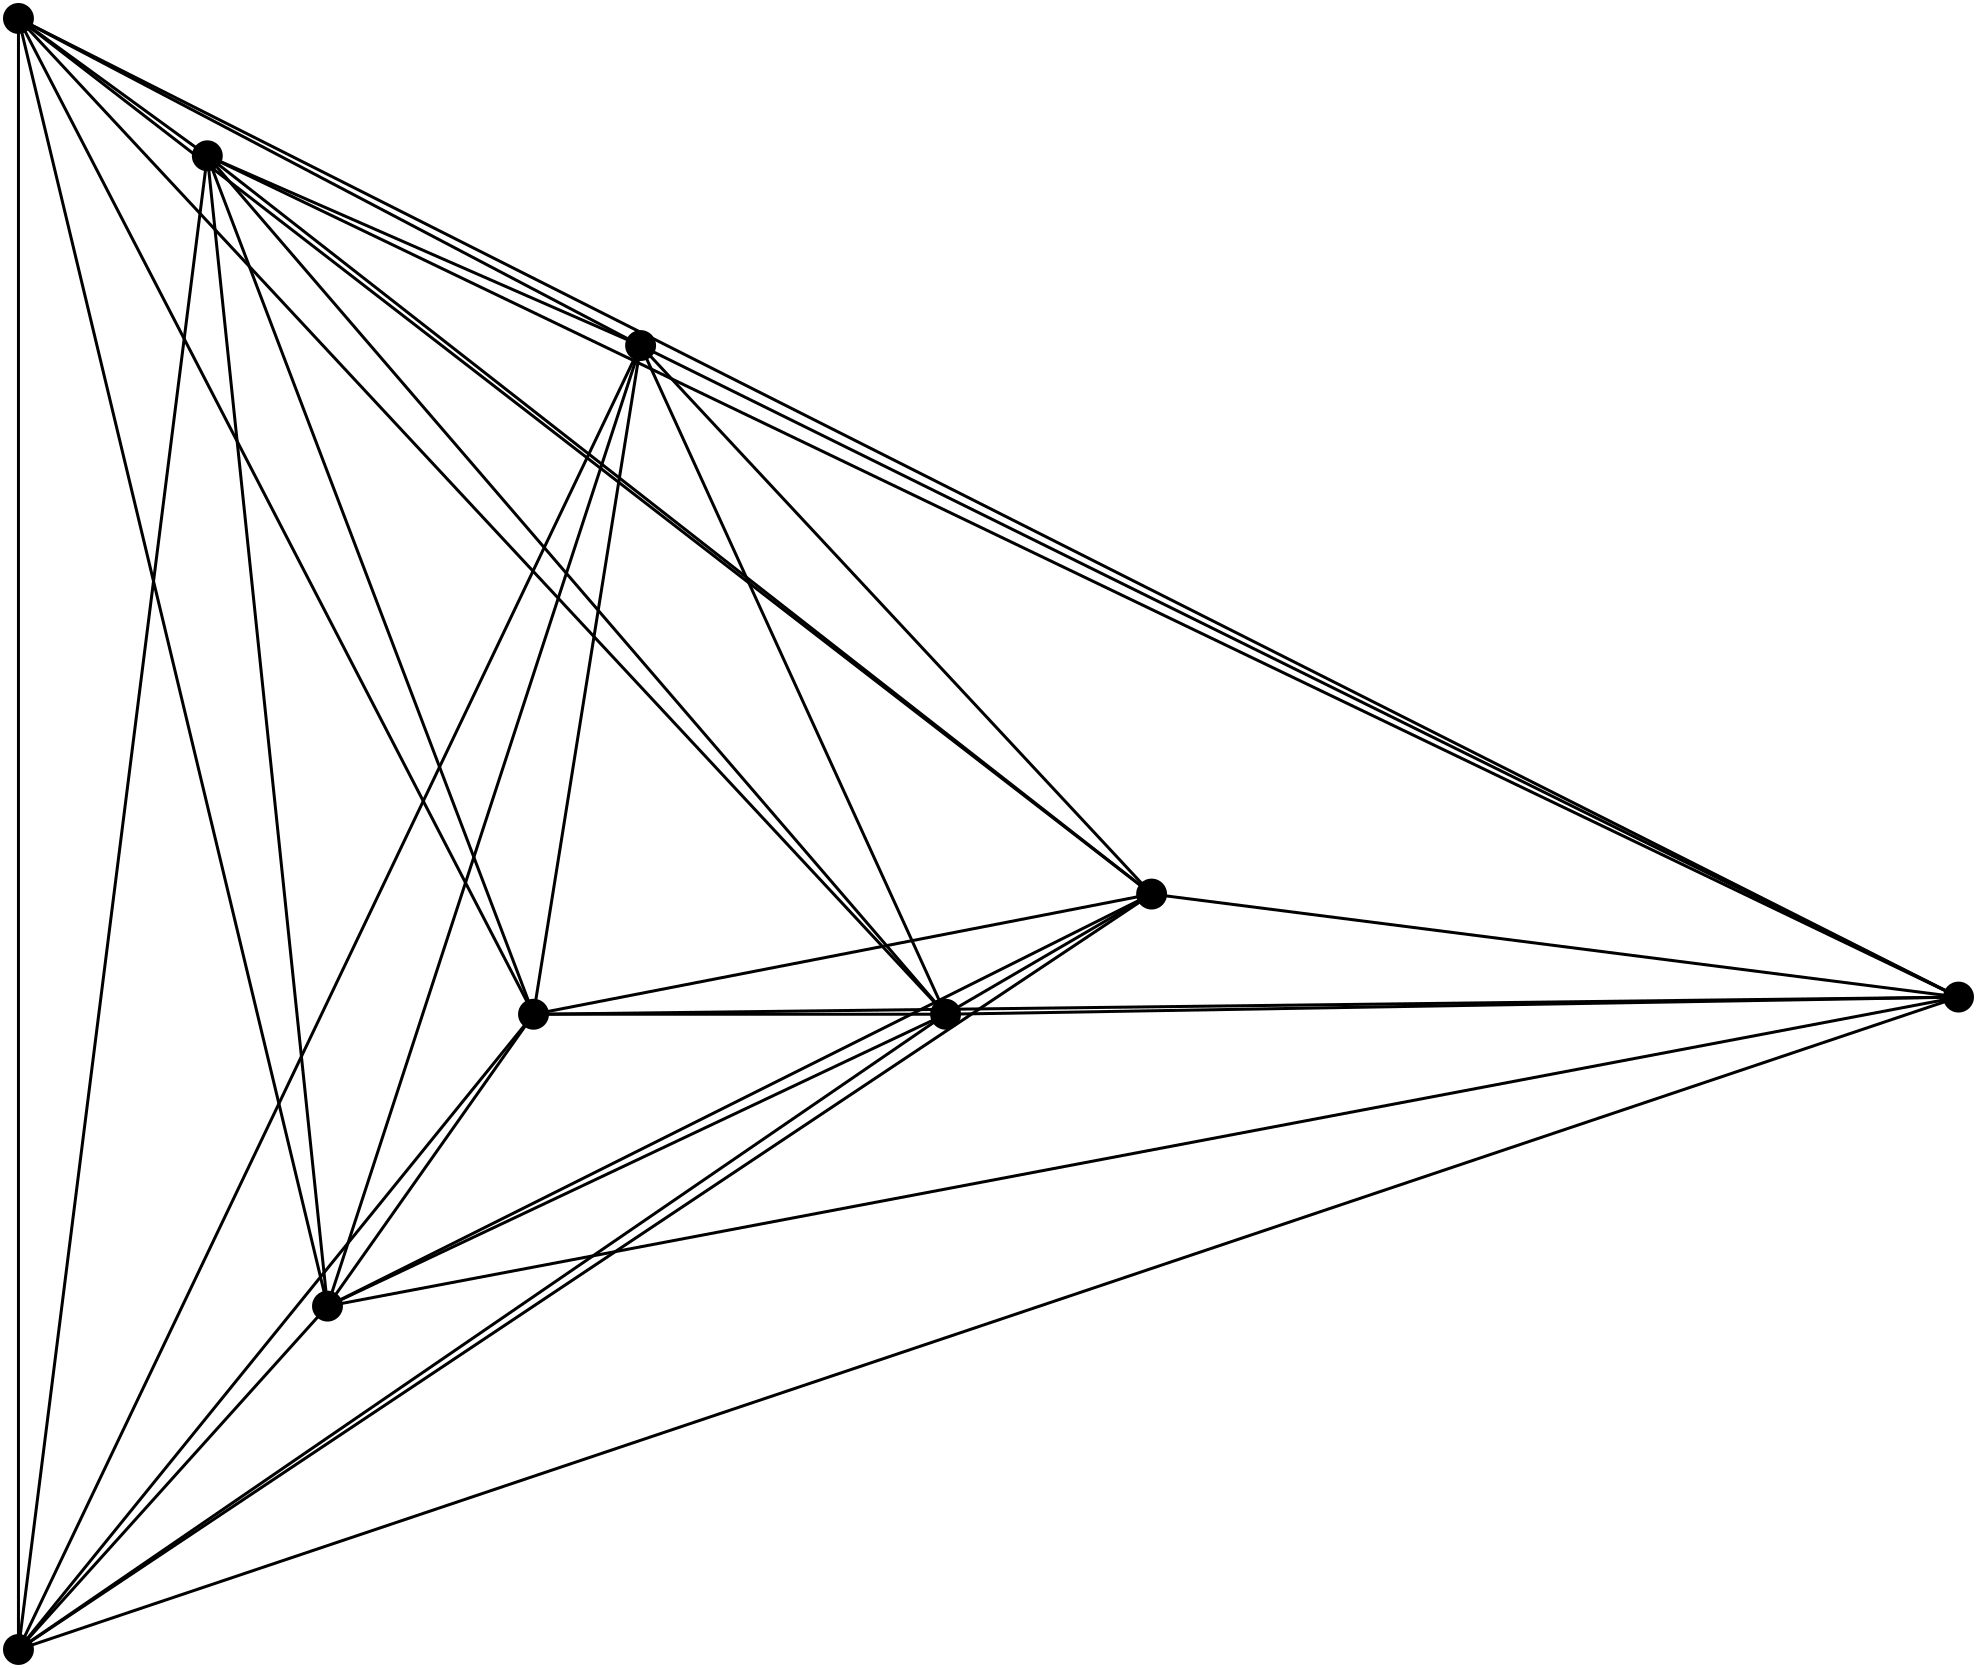
\includegraphics[width=0.8\textwidth]{k9_nomax}
  \caption{Este conjunto de puntos corresponde al tipo de orden 136764 de $n=9$.
  La gráfica completa inducida por ellos no contiene ningún thrackle máximo.}
  \label{k9_nomax}
\end{figure}
\begin{table}
  \centering
  \setlength\extrarowheight{2pt}
  \begin{tabularx}{\textwidth}{|C|l|l|l|}
    \hline
    $n$ & Tipos de orden(T.O.) & \makecell{T.O. con solo\\ un thrackle máximo} &
     \makecell{T.O. sin \\thrackles máximos\hfill} \\\hline
    3 & 1         & 1(33\%)         & 0(0\%)    \\
    4 & 2         & 0(0\%)          & 1(50\%)   \\
    5 & 3         & 0(0\%)          & 2(66\%)   \\
    6 & 16        & 1(6.25\%)       & 6(37.50\%)  \\
    7 & 135       & 7(5.18\%)       & 50(37.03\%) \\
    8 & 3315      & 208(6\%)        & 1175(35.44\%) \\
    9 & 158817    & 10547(6.64\%)   & 53758(33.84\%) \\
    10 & 14309547 & 962517(6.72\%)  & 4654339(32.52\%) \\ \hline
  \end{tabularx}
  \caption{Mostramos, para cada $3\leq n \leq 10$,
  la relación de los tipos de orden con solamente un thrackle máximo y
  los tipos de orden sin thrackles máximos.}
  \label{tabla_relacion_ot}
\end{table}

Los algoritmos que diseñamos para dar los resultados anteriores son descritos
en la sección \ref{seccion_algoritmos} para no romper con el flujo de esta
sección. Para buscar los thrackles máximos usamos el
algoritmo~\ref{algo_kthrackles}, para comparar los thrackles a pares utilizamos
el algoritmo~\ref{algo_interseccion}. La lista de tipos de orden
con un solo thrackle máximo puede ser descargada de la siguiente liga:
\url{http://computacion.cs.cinvestav.mx/~dmerinos/site/archivos_tesis/withone_ma
x.tar.gz}.
La lista de tipos de orden para los cuales no existe un thrackle máximo
está en la siguiente liga:
\url{http://computacion.cs.cinvestav.mx/~dmerinos/site/archivos_tesis/without_ma
x.tar.gz}.

Usando estos resultados podemos derivar el siguiente lema.
\begin{lemma}\label{lema:thdisjuntos}
  Sea $S$ un conjunto de puntos en posición general y sean $T_1$ y $T_2$ thrakles máximos en $K_n(S)$ con $|V(T_1)|\leq 10$
  y $|V(T_2)|\leq 10$. $T_1$ y $T_2$ tienen al menos una arista en común.
\end{lemma}
\begin{proof}
  Para cada tipo de orden con hasta diez puntos, generamos todos los thrackles
  máximos inducidos. Usando este conjunto verificamos que para cada pareja la intersección en aristas es no vacía
\end{proof}

El lema anterior implica que para $n\leq 10$ no es posible encontrar una
descomposición en thrackles máximos de tamaño
$\left\lceil\frac{n-1}{2}\right\rceil$, ya que, en dicha descomposición, los
thrackles máximos no son disjuntos a pares pero esto infringiría las
condiciones de una descomposición.
En otras palabras una descomposición por thrackles solo podría contener un
thrackle máximo. Sin embargo, es posible encontrar, a partir de una colección
de thrackles máximos, una colección de thrackles que son disjuntos.
Describimos este proceso en el siguiente lema:
% Por consecuencia es posible contar cuántas aristas son cubiertas
% por una descomposición de thrackles máximos cuyo tamaño es $\left\lceil\frac{n-1}{2}\right\rceil$.
\begin{lemma}\label{lema:existedescomp}
  Sea $\mathcal{C}=\{T_1,T_2,\dots,T_m\}$ una colección de thrackles máximos
  de $K_n$ con $|E(T_i)\cap E(T_j)| = 1$ y $ i,j \in \{1,2,\dots,m\}$.
  Existe una colección  de thrackles $\mathcal{D}$ de $K_n$ inducida por
  $\mathcal{C}$ en la que cada par de thrackles tienen intersección vacía y que
  cubre el siguiente número de aristas:
  \[\displaystyle \sum^n_{i=(n-m) + 1}i.\]
\end{lemma}
\begin{proof}
  Sea $T'_i$, con $1 \leq i \leq m$ un thrackle inducido por el siguiente
  conjunto de aristas:
  \[E(T_i) - \bigcup_{k=1}^{i-1} E(T_i)\cap E(T_k).\]

  Es decir, $T'_i$ es el thrackle que tiene todas las aristas de $T_i$
  a excepción de aquellas que $T_i$ comparte con el resto de los thrackles
  en la colección.

  Sea $\mathcal{D}=\{T'_1,T'_2,\dots,T'_m\}$. Por construcción, la intersección
  de cualesquiera dos thrackles de $\mathcal{D}$ es vacía.

  Nótese que si una arista $e$ aparece en dos thrackles de $\mathcal{C}$,
  entonces en $\mathcal{D}$, $e$ aparecerá únicamente en el thrackle con menor
  etiqueta.
  De hecho $T_1'$ tiene $n$ aristas, $T_2'$ tiene $n-1$ aristas, $T_3'$ tiene
  $n-2$ aristas y, en general, $T_i'$ tiene $n-i+1$ aristas. Como $\mathcal{D}$
  tiene $m$ thrackles el número de aristas cubiertas por $\mathcal{D}$ es
  \[ n + (n-1) + (n-2) + \cdots + (n- m + 2) + (n - m + 1).\]
  Podemos escribir esta suma como :
  \[\displaystyle \sum^n_{i=(n-m) + 1}i.\]
\end{proof}
Es importante notar que este es el máximo número de aristas que una colección
con $m$ thrackles disjuntos puede cubrir.
% Es importante notar que este es el número más grande de aristas cubiertas por
% una colección de thrackles disjuntos en aristas inducida por una colección de
% thrackles máximos, esto es debido a que en el lema~\ref{lema:thdisjuntos}
% consideramos que la intersección en aristas de dos thrackles máximos es de
% tamaño 1. No es dificil observar que si la intersección es más grande entonces
% el número de aristas cubiertas por la colección inducida es menor.

Con los lemas anteriores es posible probar que la cota inferior del
anti-thickness geométrico de $K_n$, mostrada en la ecuación,
\ref{ecuacion_cotas_atg} no es justa para toda $n$. El siguiente teorema
establece esta afirmación.
\begin{theorem}\label{teo:cotainf}
Sea $\mathcal{D}=\{T'_1,T'_2,\dots,T'_{\left\lceil\frac{n-1}{2}\right\rceil}\}$
una colección de thrackles disjuntos en aristas inducida por una colección de
$\left\lceil\frac{n-1}{2}\right\rceil$ thrackles máximos.
$\left\lceil\frac{n-1}{2}\right\rceil$ thrackles máximos son
suficientes para inducir una descomposición de $K_n$ cuando $n={3,4,6}$ y no son suficientes cuando $n={5,7,8,9,10}$.
\end{theorem}
\begin{proof}
  Se sigue del lema~\ref{lema:existedescomp}. El número de aristas cubiertas
  por $\mathcal{D}$ para cada $3\leq n \leq 10$ se muestran en la
  tabla~\ref{table:attrivialtight}. Se marcan de gris los casos en los que no es
  posible cubrir todas las aristas de $K_n$.
\end{proof}
% En la tabla~ mostramos los casos para los que la cota
% inferior del anti-thickness geométrico no es justa usando el
% lema~\ref{lema:existedescomp}.
% Es importante notar que este resultado es válido solamente cuando el dibujo de
% $K_n$ tiene al menos
% $\left\lceil\frac{n-1}{2}\right\rceil$ thrackles máximos.

\begin{table}[t]
  \centering
  \begin{tabular}{|c|c|c|c|}
    \hline
    $n$ & $\left\lceil\frac{n-1}{2}\right\rceil$ &
    $\sum^n_{i=\left(n-\left\lceil\frac{n-1}{2}\right\rceil\right) + 1}i$ &
    $\binom{n}{2}$\\[5pt] \hline\hline
    3   & 1  & 3 & 3 \\ \hline
    4   & 2  & 7 & 6 \\ \hline
    5   & 2  & \cellcolor{red!25}9 & 10 \\ \hline
    6   & 3  & 15 & 15 \\ \hline
    7   & 3  & \cellcolor{red!25}18 & 21 \\ \hline
    8   & 4  & \cellcolor{red!25}26 & 28 \\ \hline
    9   & 4  & \cellcolor{red!25}30 & 36 \\ \hline
    10  & 5  & \cellcolor{red!25}40 & 45 \\ \hline
  \end{tabular}
  \caption{ Mostramos cuántas aristas son cubiertas con una colección de
  $\left\lceil\frac{n-1}{2}\right\rceil$ thrackles máximos disjuntos en
  aristas. Se rellenan los casos en los que la colección no cubre todas las
  aristas. }
  \label{table:attrivialtight}
\end{table}

Como consecuencia del lema~\ref{lema:existedescomp} y el teorema~\ref{teo:cotainf} podemos dar una cota inferior justa para el anti-thickness geométrico de $K_n$ con $3 \leq n \leq 10$.

\begin{theorem}\label{teo:nuevacotainf}
  Sea $S$ un conjunto de $n$ puntos en el plano en posición general con $3\leq n \leq 10$, y sea $K_n(S)$ la gráfica completa inducida por $S$. El anti-thickness de $K_n(S)$:
  \begin{equation}
    At_g(K_n) \geq n - \left\lfloor\sqrt{2n+\frac{1}{4}} - \frac{1}{2}\right\rfloor.
    \label{ecuacion_cota_inf}
  \end{equation}
\end{theorem}
\begin{proof}
  Se sigue del teorema ~\ref{lema:existedescomp} que el número de aristas
  cubiertas por una colección $\mathcal{D}=\{T_1,T_2,\dots,T_m\}$ de thrackles,
  con $|E(T_i)\cap E(T_j)| = 1$, es
  \[ -\frac{1}{2}m(m-2n-1). \]
  Para saber cuántos thrackles como minimo son necesarios en la colección para
  cubrir las $\binom{n}{2}$ aristas de $K_n$, es necesario resolver la
  siguiente desigualdad otorga el resultado.
  \begin{equation}
     -\frac{1}{2}m(m-2n-1) \geq \binom{n}{2}.
     \label{ecuacion_desigualdad_cota_inf}
  \end{equation}

  De aquí se tiene que $m$ está en el siguiente intervalo:
  \[
    \frac{1}{2}\left(2n-\sqrt{8n+1} + 1\right) \leq m \leq  \frac{1}{2}\left(2n+\sqrt{8n+1} + 1\right).
  \]
  Como nosotros estamos interesados en la $m$ más pequeña para la cual se cumple la desigualdad~\ref{ecuacion_desigualdad_cota_inf}, basta con tomar el término de la izquierda para obtener el resultado deseado.
\end{proof}
  Presentamos los valores dados por la cota inferior del
  teorema~\ref{teo:nuevacotainf} en la tabla~\ref{table:atnuevacota}.
  \begin{table}[t]
    \centering
    \begin{tabular}{|c|c|c|c|}
      \hline
      $n$ & $k=n - \left\lfloor\sqrt{2n+\frac{1}{4}} - \frac{1}{2}\right\rfloor$ & $\sum^n_{i=(n-k) + 1}i$ & $\binom{n}{2}$\\[5pt] \hline\hline
      3   & 1  & 3 & 3 \\ \hline
      4   & 2  & 7 & 6 \\ \hline
      5   & 3  & 12 & 10 \\ \hline
      6   & 3  & 15 & 15 \\ \hline
      7   & 4  & 22 & 21 \\ \hline
      8   & 5  & 30 & 28 \\ \hline
      9   & 6  & 39 & 36 \\ \hline
      10  & 6  & 45 & 45 \\ \hline
    \end{tabular}
    \caption{En la tabla se muestra que la cota inferior del anti-thickness
    geométrico es justa para $3 \leq n \leq 10$. La segunda columna muestra el
    tamaño de la colección de thrackles, cuyo tamaño está dado por la cota
    inferior del anti-thickness geométrico del teorema~\ref{teo:nuevacotainf}
    para cada $n$. La tercerca columna muestra cuántas aristas cubre dicha
    colección. La cuarta columna muestra el número de aristas de $K_n$.}
    \label{table:atnuevacota}
  \end{table}

  Como consecuencia del teorema~\ref{teo:nuevacotainf} es posible obtener un valor exacto para el anti-thickness geométrico de $K_n$ en posición general.
  \begin{theorem}\label{teo:cotaexacta}
    Sea $K_n(S)$ la gráfica completa inducida por un conjunto $S$ de $n$ puntos, con $3 \leq n \leq 10$, en posición general. El anti-thickness geométrico de $K_n$ es:
    \[ At_g(K_n) = n - \left\lfloor\sqrt{2n + \frac{1}{4}} - \frac{1}{2}\right\rfloor. \]
  \end{theorem}
  \begin{proof}
    Se sigue del resultado del teorema~\ref{teo:nuevacotainf} y
    la cota superior del anti-thickness geométrico de $K_n$,
    $n - \left\lfloor\sqrt{2n + \frac{1}{4}} - \frac{1}{2}\right\rfloor $ , cuando
    $K_n$ es inducida por un conjunto de puntos en posición convexa.
  \end{proof}

  Si desearamos dar un resultado similar para $n > 10$, bastaría con generalizar el
  lema~\ref{lema:thdisjuntos}. Esto es, demostrar que cada par de thrackles máximos se
  intersecta en al menos una arista y que esto sucede para toda $n > 10$. Nosotros
  conjeturamos que este lema también se cumple para $n>10$.

  Debido a que la cota superior del anti-thickness geométrico está dada por
  el dibujo en posición convexa, en este trabajo decidimos verificar si existen
  dibujos, diferentes al convexo, para los cuales se alcanza la cota inferior
  dada por el teorema~\ref{teo:nuevacotainf}.

\section{Descomposiciones inducidas por thrackles máximos}\label{secc:descomposicion_thrackles_maximos}

  La cota superior del anti-thickness geométrico está dada por el conjunto
  de puntos en posición convexa. Sea $k=n - \left\lfloor\sqrt{2n+\frac{1}{4}} -
  \frac{1}{2}\right\rfloor$, en esta tesis verificamos que existen tipos de
  orden, que no corresponden a la posición convexa, y que inducen una gráfica
  completa cuyo anti-thickness geométrico es a lo sumo $k$.

  Para comprobar la existencia de tipos de orden con las características descritas
  anteriormente elegimos aquellos que tienen al menos $k$ thrackles
  máximos. Luego, para cada uno, analizamos todas sus colecciones de thrackles
  máximos posibles de tamaño $k$. Finalmente, para cada colección, evaluamos si
  esta cubre o no a $E(K_n)$. Cuando una colección de thrackles máximos cubre
  al conjunto de aristas de la gráfica completa, es posible inducir una descomposición
  de $K_n$ en thrackles (no necesariamente máximos) asignando cada arista de $K_n$
  a un único thrackle que la cubra. Detallamos el algoritmo para buscar
  colecciones de thrackles máximos que induzcan una descomposición en la sección
  \ref{secc:algo_descomposicion_thrackles_maximos}. La tabla~\ref{table:res_desc_th_max}
  muestra los resultados obtenidos de este análisis; observamos que para
  $n\in \{8,9,10\}$ existen tipos de orden que tienen $k$ thrackles máximos que
  pueden inducir una descomposición.


  Verificamos la optimalidad de las colecciones de thrackles máximos y encontramos
  que ninguna colección, para los tipos de orden descritos anteriormente,
  es óptima ya que en cada una existe al menos un par de thrackles cuya intersección tiene
  tamaño mayor a uno. Para este proceso utilizamos el algoritmo XY descrito en la
  sección~\ref{secc:algoritmo_optimalidad}. Este resultado nos permite dar el siguiente teorema.
  \begin{theorem}\label{teo:coleccion_optima}
    Sea $K_n(S)$ una gráfica completa inducida por un conjunto $S$ de $n$ puntos,
    con $3\leq n\leq 10$ , en posición general no convexa. No existen
    colecciones de thrackles máximos óptimas en $K_n(S)$.
  \end{theorem}
  \begin{proof}
    Se sigue de los algoritmos de la sección \ref{secc:descomposicion_thrackles_maximos}
    y la sección~\ref{secc:algoritmo_optimalidad}. El primero busca todas
    las descomposiciones posibles inducidas por colecciones de thrackles máximos.
    El segundo verifica la optimalidad de cada una de las colecciones
    encontradas por el primer algoritmo. Econtramos que no existe ninguna
    colección de thrackles máximos óptima para ningun tipo de orden diferente del convexo para
    $3\leq n\leq 10$.
  \end{proof}

  % Es importante hacer notar que encontramos configuraciones de puntos,
  % en posición no convexa, cuyo anti-thickness geométrico es $n -
  % \left\lfloor\sqrt{2n+\frac{1}{4}} - \frac{1}{2}\right\rfloor$.
  Las etiquetas de los thrackles máximos para las gráficas dadas por cada
  tipo de orden de los mostrados en la tabla~\ref{table:res_desc_th_max}, pueden
  ser consultados en el apéndice~\ref{apendice_thrackles_inducen}.

  La figura~\ref{fig:k9_descomp} muestra un ejemplo de una
  descomposición de $K_9$, en thrackles, inducida por seis
  thrackles máximos, cada thrackle es dibujado de un color diferente.

  \begin{figure}
    \centering
    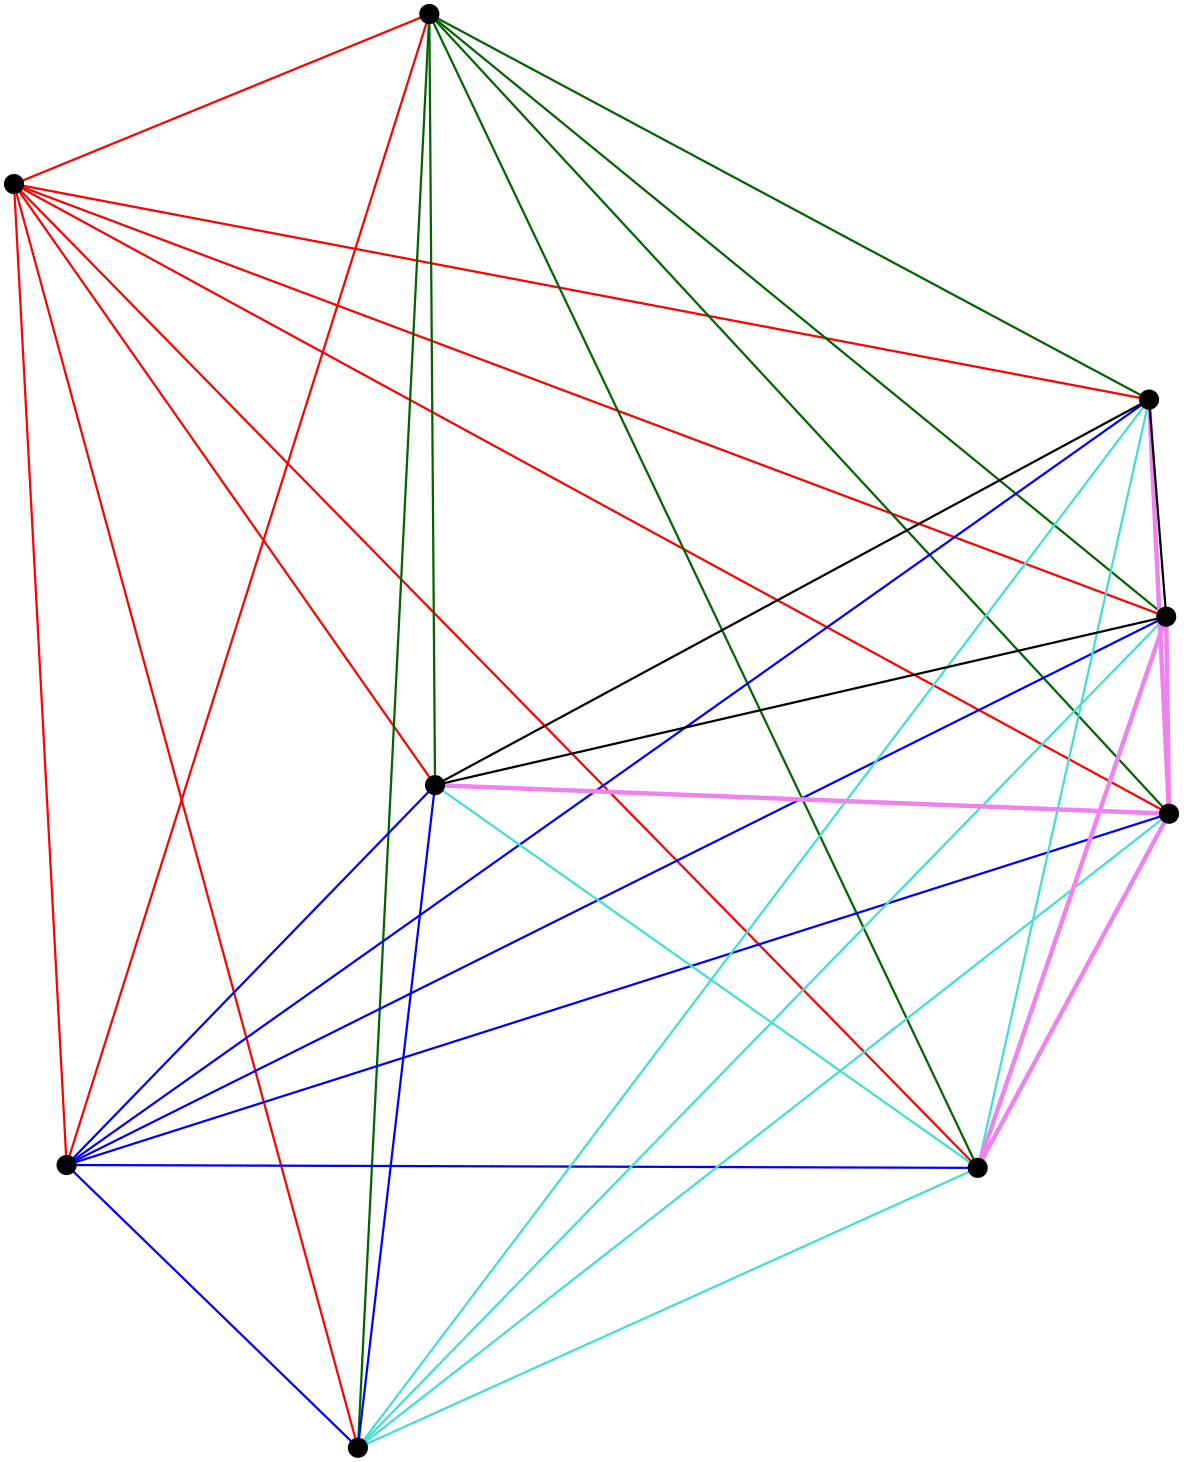
\includegraphics[width=0.7\textwidth]{k9_descomp_2}
    \caption{Una descomposición de $K_9$ en seis thrackles, la configuración de
    puntos corresponde al tipo de orden 12 con respecto de la base de datos
    de~\cite{Aichholzer2001}. El anti-thickness geométrico de $K_9$ es
    6. Esta descomposición fue inducida por una colección
    de thrackles máximos que no es óptima, es sencillo ver esto observando que
    los thrackles tienen 9,7,6,6,5 y 3 aristas respectivamente.
    Una descomposición óptima de $K_9$ tiene thrackles de tamaño 9,8,7,6,5 y 4.}
    \label{fig:k9_descomp}
  \end{figure}

  \begin{table}[htbp]
    \centering
    \setlength\extrarowheight{2pt}
    \begin{tabularx}{\textwidth}{|C|C|C|}
      \hline
      $n$   & Tipo de Orden & Tamaño de la colección \hfill $n -
      \left\lfloor\sqrt{2n+\frac{1}{4}} - \frac{1}{2}\right\rfloor$ \\ \hline\hline
      8 & 12   & 5  \\
      8 & 54   & 5  \\ \hline
      9 & 12   & 6  \\
      9 & 52   & 6  \\
      9 & 54   & 6  \\
      9 & 80   & 6  \\
      9 & 696  & 6  \\
      9 & 1080 & 6  \\
      9 & 1287 & 6  \\ \hline
     10 & 81   & 6  \\
     10 & 1328 & 6  \\
     10 & 2243 & 6  \\ \hline
    \end{tabularx}
    \caption{Tipos de orden para los que existe al menos una colección de
    $n -
    \left\lfloor\sqrt{2n+\frac{1}{4}} - \frac{1}{2}\right\rfloor$ thrackles máximos que cubren a $K_n$.}
    \label{table:res_desc_th_max}
  \end{table}

  Para los casos de $n \in \{3,4,\dots,7\}$ no existe ninguna
  colección de $k$ thrackles máximos que pueda inducir una descomposición de
  $K_n$. Esto es porque, para ninguno de los tipos de orden, en este rango de $n$,
  existe una colección de thrackles máximos que cubran las aristas de $K_n$.
  Para estos valores de $n$ buscamos, de manera manual, una descomposición
  con ese número de thrackles (no necesariamente máximos).
  La figura~\ref{fig:descomposicionesk4_k9}
  muestra para cada color de $n$ con $3\leq n\leq 7$, dibujos cuyo anti-thickness
  es igual a la cota inferior del teorema~\ref{teo:nuevacotainf}. De esto se sigue
  que el anti-thickness geométrico de $K_n$, con $ 3 \leq n \leq 7$, es a lo
  sumo $n - \left\lfloor\sqrt{2n+\frac{1}{4}} - \frac{1}{2}\right\rfloor$.
  Como resultado podemos decir que el anti-thickness geométrico de $K_n$, con $ 3\leq n \leq 10$
  es exactamente $n - \left\lfloor\sqrt{2n+\frac{1}{4}} - \frac{1}{2}\right\rfloor$.

  \begin{figure}[htpb]
    \centering
    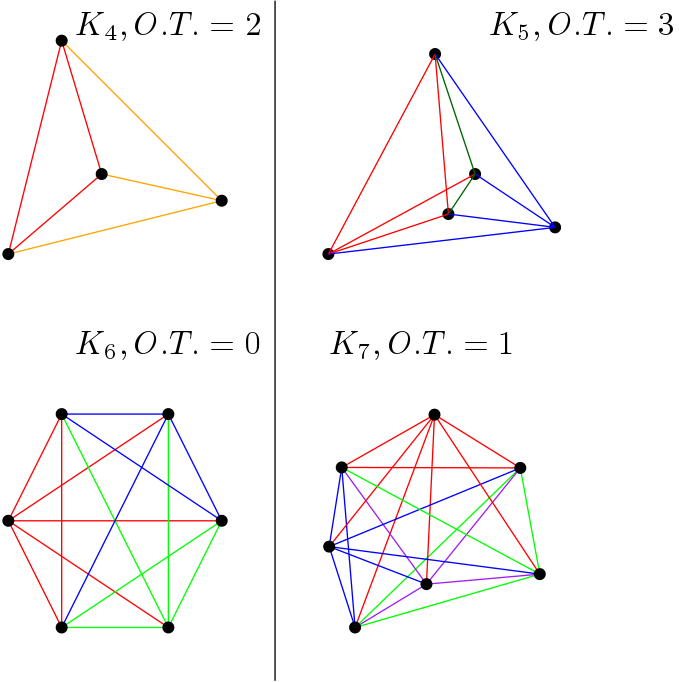
\includegraphics[width=0.7\textwidth]{descomposiciones_K49.png}
    \caption{Mostramos posibles descomposiciones de la gráfica completa con
    hasta 7 vértices. Las descomposiciones tienen exáctamente el número de
    thrackles establecido por la cota inferior del
    teorema~\ref{teo:nuevacotainf}. Estas configuraciones de puntos, a excepción de $K_6$, son
    diferentes de la posición convexa. Los tipos de orden correspondientes a cada dibujo están
    indicados en la figura como $O.T.$}
    \label{fig:descomposicionesk4_k9}
  \end{figure}

  En la siguiente sección analizamos, para $ 3\leq n\leq 9$, cómo
  se comporta la intersección de thrackles, no necesariamente máximos, de los
  dibujos de $K_n$.


  \section{Intersección de thrackles de $K_n$ con $3\leq n \leq 9$.}
    \chaptermark{$gat(n)$ exacto para $3\leq n \leq 9$.}

    % Debido a que los resultados de la sección X son aplicables solamente para los tipos de orden con al menos un determinado número
    % de thrackles máximos, decidimos analizar el anti-thickness geométrico para los demás tipos de orden. Para realizar este análisis
    % tratamos de responder la siguiente pregunta: ¿Podemos encontrar, para algún tipo de orden, una descomposición en thrackles cuyo
    % tamaño sea menor a la cota superior de $At_g(K_n)$? En general, esto no es posible.
    Debido al resultado del teorema~\ref{teo:coleccion_optima} establecido
    en la sección~\ref{secc:descomposicion_thrackles_maximos} decidimos estudiar
    la existencia de colecciones de thrackles, no necesariamente máximos,
    cuya intersección a pares es vacía y que además puedan cubrir las arsitas
    de $K_n$. Para explicar este proceso primero es necesario definir una
    \emph{partición de un entero}.

    \begin{definition}{\emph{Partición de un entero.}(~\cite{Knuth2011})}
      Una partición de un entero $n$ es una colección de enteros
      no negativos $P = \{a_1, a_2, \dots, a_m\}$ tales que
      $a_1 \geq a_2\geq \dots \geq a_m$ y $a_1 + a_2 + \dots + a_m = n$.
    \end{definition}
    %
    % Nosotros utilizamos las particiones de enteros como guía para construir una
    % descomposición y construimos un algoritmo que intenta encontrar dichas
    % descomposiciones en thrackles.

    Es posible usar ciertas particiones de un entero como guía para buscar
    descomposiciones en thrackles de $K_n$. Por ejemplo, si  deseamos obtener
    una descomposición en thrackles de $K_4$, entonces necesitamos cubrir
    seis aristas. El entero 6 tiene once particiones, tres de ellas son:
    $\{4,2\},\{2,2,2\},\{3,1,1,1\}$. Las cuales pueden traducirse a tres diferentes
    descomposiciones, la partición $\{4,2\}$ se traduce en una descomposición
    con un thrackle con cuatro aristas y uno de dos aristas, la partición
    $\{2,2,2\}$ se traduce en una descomposición con 3 thrackles con dos
    aristas cada uno, la partición $\{3,1,1,1\}$ se traduce a una descomposición
    con un thrackle con tres aristas y tres thrackles con una arista. Debido a que
    nosotros estudiamos descomposiciones de tamaño estrictamente menor
    a la cota superior del anti-thickness geométrico, que es:
    $n - \left\lfloor\sqrt{2n+\frac{1}{4}} - \frac{1}{2}\right\rfloor$, y
    como en una descomposición solamente puede existir un thrackle máximo, es
    posible imponer condiciones sobre las particiones de enteros para
    las particiones que usaremos. Nos referimos a estas como
    \emph{particiones válidas de un entero}.
    \begin{definition}{\emph{Partición válida de un entero.}}
      Sea $K_n(S)$ la gráfica completa inducida por un conjunto $S$ de $n$
      puntos en posición general.
      Una partición $P=\{a_1,a_2,\dots,a_m\}$ es válida si cumple
      con las siguientes condiciones:
      \begin{itemize}
        \item Si $a_1$ es igual a $n$ entonces solo existe una ocurrencia de $a_1$ en $P$.
        \item La suma $a_1 + a_2 + \dots + a_m = \binom{n}{2}$.
        \item $m < n - \left\lfloor\sqrt{2n+\frac{1}{4}} - \frac{1}{2}\right\rfloor$.
      \end{itemize}
    \end{definition}

    No existe una formula cerrada para conocer el número de particiones de
    algún entero $n$. Sin embargo, si se considera a las composiciones
    de un entero $n$ como las secuencias de enteros positivos en donde el orden
    importa, es decir, dos composiciones diferentes del entero 3 serían $\{2,1\}$
    y $\{1,2\}$, entonces podemos acotar el espacio de búsqueda de las particiones
    de un entero. Como el número de composiciones para un entero $n$ es $2^{n-1}$
    podemos decir que existen a lo sumo $O(2^{n-1})$ particiones para el
    mismo entero $n$.

    Usando esta definición generamos las particiones válidas para todo entero
    $x\in \left\{ \binom{3}{2}, \binom{4}{2}, \cdots, \binom{10}{2}\right\}$.
    En ~\cite{Knuth2011} se ofrece un algoritmo para
    generar las particiones de algún entero $n$. Nosotros utilizamos
    dicho algoritmo en este trabajo modificandolo para que genere solamente
    particiones válidas de un entero. Discutimos con más detalle el algoritmo en
    la sección~\ref{secc:algo_particiones_validas}.
    La tabla~\ref{tabla:particionesk8k9} muestra las particiones generadas por el
    algoritmo; es posible observar que para $x\in \left\{\binom{3}{2},\binom{4}{2}
    \cdots,\binom{7}{2}\right\}$ no existen particiones válidas, esto reafirma,
    para $ 3\leq n\leq 7$ el resultado del teorema~\ref{teo:nuevacotainf}
    que establece una cota inferior para el anti-thickness geométrico de $K_n$. Por otro lado,
    no generamos las particiones para $K_10$ ya que debido al tamaño de los archivos binarios
    generados con el algoritmo de búsqueda de thrackles no fue posible diseñar un algoritmo durante
    el tiempo del desarrollo de este trabajo.
    \begin{table}[t]
      \centering
      \begin{tabular}{|c|c|}
        \hline
        $n$                       & Particiones de $\displaystyle\binom{n}{2}$ \\ \hline\hline
        \multirow{2}{*}{$ 8 $}    & $\{8,7,7,6\}$ \\ \cline{2-2}
                                  & $\{7,7,7,7\}$ \\ \hline
        \multirow{11}{*}{$ 9 $}   &$\{9,8,8,8,3\}$ \\ \cline{2-2}
                                  &$\{9,8,8,7,4\}$ \\ \cline{2-2}
                                  &$\{9,8,8,6,5\}$ \\ \cline{2-2}
                                  &$\{9,8,7,7,5\}$ \\ \cline{2-2}
                                  &$\{9,8,7,6,6\}$ \\ \cline{2-2}
                                  &$\{9,7,7,7,6\}$ \\ \cline{2-2}
                                  &$\{8,8,8,8,4\}$ \\ \cline{2-2}
                                  &$\{8,8,8,7,5\}$ \\ \cline{2-2}
                                  &$\{8,8,8,6,6\}$ \\ \cline{2-2}
                                  &$\{8,8,7,7,6\}$ \\ \cline{2-2}
                                  &$\{8,7,7,7,7\}$ \\ \hline
      \end{tabular}
      \caption{Particiones de enteros del número de aristas de $K_8$ y de $K_9$. }
      \label{tabla:particionesk8k9}
    \end{table}

    Usando las particiones de la tabla~\ref{tabla:particionesk8k9} diseñamos
    una serie de procedimientos que buscan thrackles disjuntos usando las particiones como guía.
    Como hay cerca de 14 procedimientos para realizar esta tarea, expondremos solamente
    uno de ellos en el algoritmo YX de la sección~\ref{secc:descomposiciones_particiones}, los
    otros algoritmos son similares a este. Como resultado de estos procedimientos podemos dar el
    siguiente teorema:
    \begin{theorem}
      Sea $P=\{a_1,a_2,\dots,a_m\}$ una partición válida para $K_8$ o para $K_9$. No existe, para
      ningún dibujo diferente del convexo, una colección $\mathcal{D}=\{T_1,T_2,\dots,T_m\}$ de
      thrackles disjuntos tales que $|E(T_1)|=a_1,|E(T_2)|=a_2,\dots,|E(T_m)|=a_m$.
    \end{theorem}
    \begin{proof}
      Se sigue del resultado de la ejecución de los algoritmos para evaluar colecciones de
      thrackles. Los algoritmos encuentran que, para ninguna partición de la
      tabla~\ref{tabla:particionesk8k9}, existe una colección de thrackles disjuntos cuyo número de
      aristas corresponde a las particiones válidas de $K_8$ y $K_9$.
    \end{proof}

\section{Algoritmos}\label{seccion_algoritmos}
En esta sección presentamos los algoritmos usados en el trabajo. Empezamos
describiendo el algoritmo para encontar thrackles de cualquier tamaño dado
un conjunto de puntos en posición general. Después hablamos del algoritmo
usado para encontrar la intersección de dos thrackles con el mismo número de
aristas. Luego...Finalmente...


\subsection{Algoritmo para encontrar thrackles con $k$
  aristas}\label{seccion_algoritmo_kthrackles}
  A continuación presentamos el algoritmo para encontrar thrackles de tamaño
  $k$, donde $k$ es dada. Usando este algoritmo se resuelve el problema de
  encontrar todos los thrackles con $k$ aristas para todos los tipos de orden
  de alguna $n$. El algoritmo recibe como entrada los valores de $n$ y $k$
  donde $1 \leq k \leq n$. Como salida se entrega el número de thrackles con
  $k$ aristas y se generan archivos binarios con los datos de los thrackles
  encontrados.

  Este algoritmo fue implementado en el lenguaje \texttt{C++}; utilizamos una
  estructura de datos llamada vector. Un vector es un contenedor que representa
  a un arreglo que puede cambiar de tamaño. El vector puede ser accedido igual
  que un arreglo (usando el operador \texttt{[]}) con la misma eficiencia.

  Este algoritmo requiere tres pasos de preparación para funcionar. Describimos estos pasos a continuación. Para cada tipo de orden $S$:
  \begin{enumerate}
    \item Leer y almacenar el archivo que contiene el tipo de orden $S$.
    Los puntos se almacenan en un vector de tamaño $n$ donde cada elemento es
    un objeto que contiene las coordenadas $x$ y $y$ de cada uno de los puntos
    de $S$.
    \item Generar y almacenar las aristas de la gráfica completa inducida por
    $S$. Para cada punto almacenado $p_i$ creamos todas las aristas (no
    dirigidas) que tienen como punto inicial a $p_i$ y como punto final a $p_j$
    donde $ i+1 \leq j \leq n$.
    Las aristas son almacenadas en un vector de tamaño $\binom{n}{2}$ y las
    etiquetamos con enteros desde $0$ hasta $\binom{n}{2}-1$.
    \item \label{paso3}Construir la \emph{matriz de disyunción}.
    Construimos una matriz binaria de $\binom{n}{2}\times \binom{n}{2}$. La
    matriz es almacenada en un arreglo de arreglos convencional. Cada
    indice de las filas y de las columnas representa a cada una de las aristas
    de $K_n(S)$ de manera tal que la fila $i$ representa a la arista que tiene
    la etiqueta $i$, consideramos que la enumeración de las filas y columnas de
    la matriz empieza desde $0$, por lo que $i \in [0,\binom{n}{2}-1]$. Esto ocurre de la misma manera para las columnas.

    La matriz de disyunción tiene un 0 en la entrada $(i,j)$ si las aristas $i$ y $j$ se cruzan o comparten un vértice y tiene un 1 en en la entrada $(i,j)$ si las aristas $i$ y $j$ son totalmente disjuntas. Es decir, construimos la
    matriz de adyacencia de la gráfica $D(S)$.
  \end{enumerate}

  A continuación describimos el algoritmo que usamos para encontrar thrackles
  de tamaño $k$, este algoritmo usa la matriz de disyunción construida en el
  paso~\ref{paso3}. El pseudocódigo se encuentra en el
  algoritmo~\ref{algo_kthrackles}.

  El algoritmo que diseñamos utiliza la técnica de \emph{backtracking},
  recordemos que se desea encontrar todos los thrackles de tamaño $k$. Para
  nosotros, un solo thrackle de tamaño $k$ es una solución. Una solución es
  almacenada en un vector $C$. En cada entrada del vector se almacenan las etiquetas que conforman un thrackle con $k$ aristas.

  En cada iteración, el algoritmo verifica si ya se han encontrado $k$ aristas
  que se intersectan a pares, para evaluar la intersección se usa la matriz de
  disyunción.

  Supongamos que el vector $C$ tiene entradas desde $C[0]$ hasta $C[j]$ y que
  $j+1 < k$. Esto quiere decir que las aristas $C[0],C[1],\dots,C[j]$ forman un
  thrackle con $j+1$ aristas. El algoritmo buscaría extender el tamaño de este
  thrackle en uno. Para esto hacemos $C[j+1]=C[j]+1$ y verificamos que $C[j+1]$
  intersecte a $C[0],C[1],C[2],\dots,C[j-1],C[j]$. Si lo hace, entonces
  $C[j+1]$ forma parte del thrackle y ahora el thrackle tiene $j+2$ aristas. En
  caso contrario hacemos $C[j+1]=C[j+1]+1$, es decir, se descarta la arista que
  estaba en $C[j+1]$ y es reemplazada por la arista subsecuente en la
  etiquetación.

  Si en algún momento la entrada $C[j]$ tiene un valor mayor o igual a
  $\binom{n}{2}$, esto es, que ya agotó los valores posibles para representar
  alguna arista en $K_n$, entonces, se incrementa el valor de la entrada
  $C[j-1]$ en uno y se continua la verificación a partir de esta entrada. Esto
  permite que el algoritmo realice el proceso de \emph{backtracking}.

  Si el vector $C$ tiene $k$ entradas, es decir, encontró un thrackle con $k$
  aristas entonces almacenamos el contenido del vector $C$ en una lista de
  vectores. Como ya se encontró una solución y esta ha sido procesada, para
  buscar la siguiente solución, le indicamos al algoritmo que el thrackle tiene
  actualmente tamaño $k-1$, provocando así que en la siguiente iteración se
  busque incrementar el tamaño del thrackle en uno.

  Es posible observar un ejemplo de cómo se llena el vector $C$ en una
  ejecución del algoritmo en la figura~\ref{fig:ejemplo_backtracking}.

  En el  inicio de la ejecución del algoritmo, el vector $C$ está vacío, es
  decir, que  todas sus entradas tienen un valor nulo a excepción de la primera
  entrada $C[0]$ cuyo valor es 0. Esta inicialización es necesaria para poner
  en marcha el algoritmo. De esta manera, el algoritmo encuentra primero todos
  los thrackles que contengan a la arista con etiqueta 0. Una vez que la
  posición $C[0]$ tenga un valor mayor o igual a $\binom{n}{2}$, el valor de
  $C[0]$ será igual a 1. Esto hará que el algoritmo busque los thrackles que
  contengan a la arista con etiqueta 1. Este proceso se repite para todos los
  valores entre $0$ y $\binom{n}{2}-1$.

  Este algoritmo solamente genera soluciones que son efectivamente thrackles.
  Puesto que en $C$ solo se avanza a la siguiente posición
  cuando se encuentra que la arista de la posición actual intersecta a las
  aristas anteriormente establecidas. Además, el algoritmo genera todos los
  thrackles con $k$ aristas. Si no lo hiciera significaría que no evaluó
  determinada combinación de aristas, lo cual no es posible. El algoritmo
  evalúa virtualmente todas las combinaciones posibles de aristas ya que, para
  cada entrada $1\leq j\leq k$, $C[j]$ toma valores en el rango
  $\left[C[j-1],\binom{n}{2}\right]$. Para el caso particular de la entrada
  $C[0]$, se toman los valores en el rango $\left[ 0, \binom{n}{2}\right]$. Las
  combinaciones que no se evalúan son aquellas que no hace sentido evaluar,
  estas son las combinaciones que contienen al menos una arista disjunta de
  alguna de las otras aristas de la combinación.

  \begin{figure}[htpb]
    \centering
    \begin{tikzpicture}[
     node distance = 15mm and 1mm,
       start chain = A going right,
       start chain = R going right,
       nd/.style = {draw=none, fill=none, on chain=A, minimum width =10mm},
       mpn/.style args = {#1/#2/#3/#4}{draw,
       rectangle split, rectangle split horizontal,
       rectangle split parts=4,
       on chain=A,
       node contents={ \nodepart{one}    $#1$
                       \nodepart{two}    $#2$
                       \nodepart{three}  $#3$
                       \nodepart{four}   $#4$}
                                   },
       root/.style args = {#1/#2/#3/#4}{draw,
       rectangle split, rectangle split horizontal,
       rectangle split parts=4,
       on chain=R,
       node contents={ \nodepart{one}    $#1$
                       \nodepart{two}    $#2$
                       \nodepart{three}  $#3$
                       \nodepart{four}   $#4$}
                                   },
                           ]


       \node[mpn=0/NIL/NIL/NIL]; %A1
       \node[mpn=1/NIL/NIL/NIL]; %A2
       \node[mpn=2/NIL/NIL/NIL]; %A3
       \node[nd]{...};           %A4
       \node[mpn=0/1/NIL/NIL, below=of A-1];   %A5
       \node[mpn=0/2/NIL/NIL, right=of A-5]; %A6
       \node[mpn=0/1/2/NIL, below=of A-5 ]; %A7
       \node[nd,right=of A-6]{...}; %A8
       \node[mpn=0/1/3/NIL, right=of A-7];  %A9
       \node[mpn=0/1/3/4, below=of A-9, fill=gray]; %A10
       \node[mpn=0/1/3/5, right=of A-10, fill=gray]; %A11
       \node[nd,right=of A-11]{...}; %A12
       \node[nd, right=of A-6]{...}; %A13
        \node[nd, right=of A-9]{...}; %A14
        \node[nd, below=of A-4]{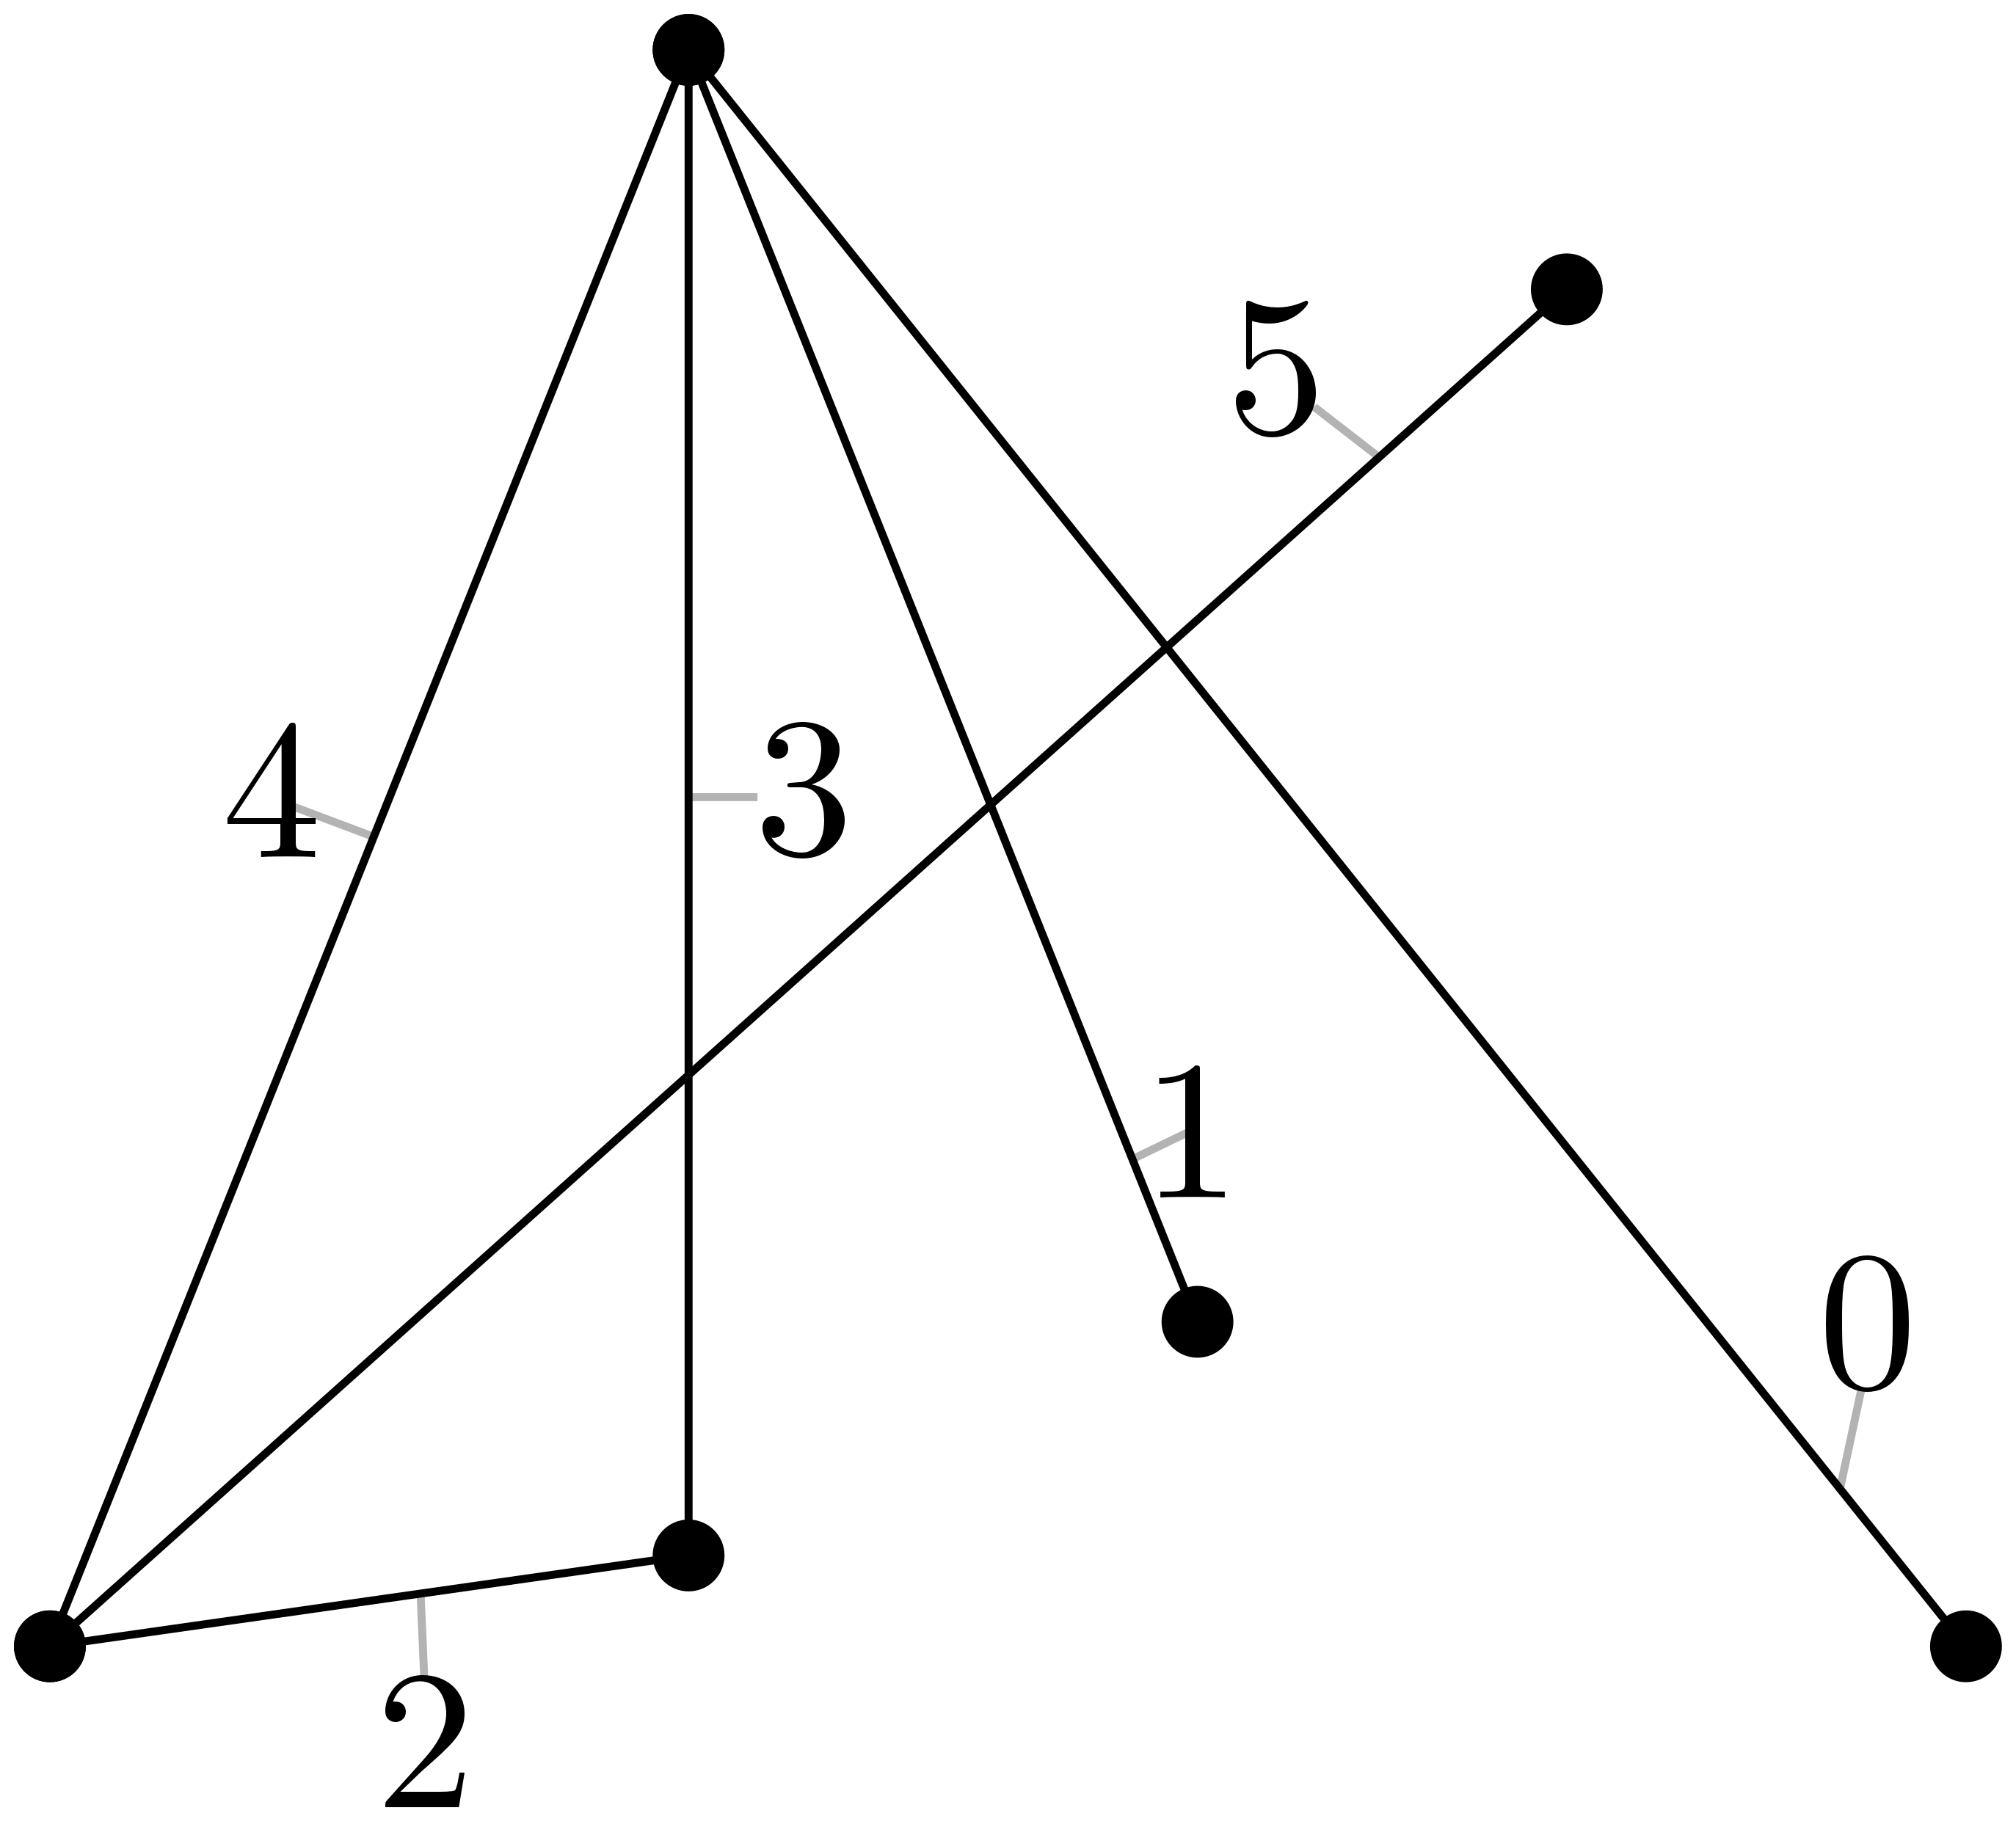
\includegraphics[width=0.4\textwidth]{ejemplo_backtracking}};
       %\draw{...}
       %
       \node[root=NIL/NIL/NIL/NIL, %ROOT.
             above=of $(A-1.north west)!0.5!(A-4.north east)$];

       \foreach \i in {1,...,3}
       \draw[-Stealth, semithick, shorten >=1mm, shorten <=1mm]
           (R-1.south) -- (A-\i.north);
       \draw[-Stealth, semithick, shorten >=1mm, shorten <=1mm]
           (R-1.south) -- (A-4.north);
       \draw[-Stealth, semithick, shorten >=1mm, shorten <=1mm]
           (A-1.south) -- (A-5.north);
       \draw[-Stealth, semithick, shorten >=1mm, shorten <=1mm]
           (A-1.south) -- (A-6.north);
       \draw[-Stealth, semithick, shorten >=1mm, shorten <=1mm]
           (A-1.south) -- (A-8.north);
       \draw[-Stealth, semithick, shorten >=1mm, shorten <=1mm]
           (A-5.south) -- (A-7.north);
       \draw[-Stealth, semithick, shorten >=1mm, shorten <=1mm]
           (A-5.south) -- (A-9.north);
       \draw[-Stealth, semithick, shorten >=1mm, shorten <=1mm]
           (A-5.south) -- (A-14.north);
       \draw[-Stealth, semithick, shorten >=1mm, shorten <=1mm]
           (A-9.south) -- (A-10.north);
       \draw[-Stealth, semithick, shorten >=1mm, shorten <=1mm]
           (A-9.south) -- (A-11.north);
       \draw[-Stealth, semithick, shorten >=1mm, shorten <=1mm]
           (A-9.south) -- (A-12.north);
    \end{tikzpicture}
    \caption{La figura muestra un ejemplo de cómo cambia el vector $C$ cuando se busca un thrackle
    con 4 aristas para alguna $n>5$. Solamente se representan algunas instancias del vector $C$.
    En este ejemplo suponemos que las aristas con etiqueta 1 y 2 no se
    intersectan. Es posible observar que cuando $C=[0,1,2,NIL]$ no se generan, debajo de ese nivel,
    combinaciones con las etiquetas 1 y 2. Se marcan de fondo gris las soluciones encontradas.
    En el lado derecho presentamos un dibujo de una gráfica en la que se buscan los thrackles con
    4 aristas.}
    \label{fig:ejemplo_backtracking}
  \end{figure}

  \algblockdefx[NAME]{}{OTHEREND}%
  [1]{Until (#1)}
  \begin{algorithm}[htpb]
    \begin{algorithmic}[1]
      \Procedure{EncontrarThrackleK}{$n,k$}
      \State Sea $C$ un vector de tamaño $k+1$.
      \State $C[0]\gets 0$
      \State $C[i]\gets NIL$ para $ 1 \leq i \leq k+1$
      %\State $C[1]\gets $
      \State \texttt{inters\_flag} $\gets$ \texttt{true}
      \State \texttt{curr\_size} $\gets 0$
      \While{$C[0] < \binom{n}{2}$}
      \While{\texttt{curr\_size}$<k$}
      \State \texttt{inters\_flag} $=$ \texttt{true}
      \If{$C[\text{\texttt{curr\_size}}] \geq \binom{n}{2}$}
        \State \texttt{curr\_size} $\gets$  \texttt{curr\_size} $-1$
        \If{\texttt{curr\_size} $<0$}
        \State \Return \texttt{thrackle\_counter}
        \EndIf
        \State $C[\text{\texttt{curr\_size}}]\gets C[\text{\texttt{curr\_size}}]+1$
        \State \textbf{continue}
      \EndIf
      \For{$i\gets 0 \dots \text{\texttt{curr\_size}}-1$}
        \State \texttt{inters\_flag}=\texttt{inters\_flag} $\&\&$ \texttt{matrix}$[C[i]][C\text{\texttt{curr\_size}}]$
      \EndFor
      \If{\texttt{inters\_flag} $==$ \texttt{False}}
        \State $C[\text{\texttt{curr\_size}}] \gets C[\text{\texttt{curr\_size}}] + 1$
      \Else
        \If{\texttt{curr\_size}$+1==k$}
          \State \texttt{thrackle\_counter} $\gets$ \texttt{thrackle\_counter} + 1
          \State Almacenar $C$ en una lista de vectores.
          \State \textbf{continue}
        \EndIf
      \EndIf
      \EndWhile
      \State $C[\text{\texttt{curr\_size}}+1] \gets C[\text{\texttt{curr\_size}}] + 1$
      \State \texttt{curr\_size} $\gets$ \texttt{curr\_size} $+1$
      \EndWhile
      \EndProcedure
    \end{algorithmic}
    \caption{Algoritmo para encontrar todos los thrackles de tamaño $k$.}
    \label{algo_kthrackles}
  \end{algorithm}

  % La información de los thrackles encontrados para cada $3\leq n \leq 10$ es
  % almacenada en archivos binarios de nombre \texttt{n\_k\_All\_bool.ths}
  % donde \texttt{k} es el número de aristas para cada thrackle. El archivo binario
  % tiene la siguiente estructura:
  % \begin{enumerate}
  %   \item Tipo de orden escrito como caracter binario de tipo \texttt{uint16\_t}.
  %   \item Número de thrackles de tamaño $k$ para determinado tipo de orden
  %   escrito como caracter binario de tipo \texttt{uint16\_t}.
  %   \item Para cada thrackle, se escribe una lista de $\binom{n}{2}$ caracteres
  %   binarios que representan cada una de las aristas, si el $j$-ésimo elemento de
  %   la lista tiene un $0$ en el $i$-ésimo caracter entonces el thrackle $j$
  %   tiene la arista $i$. Cada caracter de la lista está escrito con un caracter
  %   de tipo \texttt{char}.
  % \end{enumerate}
  %
  % La figura~\ref{fig:binaryfile} muestra un ejemplo de la sintaxis
  % descrita anteriormente.
  % \begin{figure}[htpb]
  %   \centering
  %   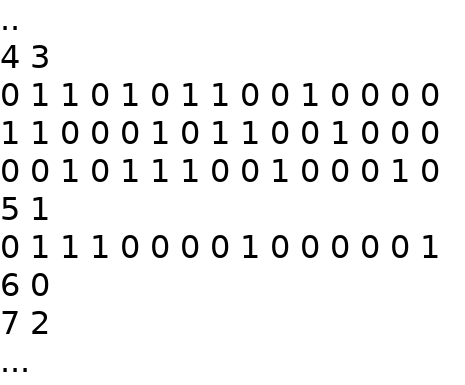
\includegraphics[width=0.4\linewidth]{binaryfile}
  %   \caption{Un segmento de un archivo binario, en este ejemplo $n=6$ y $k=6$.
  %   La primera línea indica que para el tipo de orden $4$ existen $3$ thrackles
  %   con $6$ aristas. Las siguientes 3 lineas indican las aristas de cada uno
  %   de los thrackles con un $1$. Después, para el tipo de orden 5, existe un
  %   thrackle, para el tipo de orden 6 no existen thrackles con 6 aristas. El
  %   archivo binario continua de esta manera para cada uno de los tipos de orden
  %   para $n=6$. Este ejemplo no representa necesariamente los datos reales
  %   encontrados en este trabajo para $n=6$.}
  %   \label{fig:binaryfile}
  % \end{figure}

  Los datos de los thrackles máximos encontrados para cada $ 3\leq n \leq 9$
  pueden ser descargados de la siguiente liga:
  \url{http://computacion.cs.cinvestav.mx/~dmerinos/site/archivos_tesis/3to9.tar.gz}
  el archivo para $n=10$, separado debido a su tamaño,
   puede ser descargado de la siguiente liga:
  \url{http://computacion.cs.cinvestav.mx/~dmerinos/site/archivos_tesis/10.tar.gz}

\subsection{Algoritmo para la intersección de dos thrackles}
  Dados dos thrackles con el mismo número de aristas, codificados como cadenas
  de enteros, aprovechamos el ordenamiento lexicográfico para hacer la
  operación de intersección de thrackles en tiempo lineal.
  Sea $A$ y $B$ dos vectores que representan las aristas de dos thrackles, con
  $|A|=|B|=k$. El algoritmo~\ref{algo_interseccion} entrega la intersección de $A$ y $B$ y la
  almacena en un conjunto $C$. Este algoritmo es secuencial y visita en el peor caso todas las
  entradas de los dos vectores.
  \begin{algorithm}[htpb]
    \begin{algorithmic}[1]
      \Procedure{ThrackleIntersection}{$A,B,C$}
      \State $i\gets 0$
      \State $j\gets 0$
      \While{$i<k$ and $j<k$}
        \If{$A[i] < B[j]$}
          \State $i\gets i+1$
          \State \textbf{continue}
        \EndIf
        \If{$A[i]==B[j]$}
          \State $C\gets C\cup \{A[i]\}$
          \State $i\gets i+1$
          \State $j\gets j+1$
          \State \textbf{continue}
        \EndIf
        \If{$A[i]>B[j]$}
          \State $j\gets j+1$
          \State \textbf{continue}
        \EndIf
      \EndWhile
      \EndProcedure
    \end{algorithmic}
    \caption{Intersección de dos conjuntos ordenados en tiempo lineal.}
    \label{algo_interseccion}
  \end{algorithm}

\subsection{Algoritmo para encontrar colecciones de thrackles máximos que
inducen descomposiciones en thrackles de $K_n$}\label{secc:algo_descomposicion_thrackles_maximos}
  El algoritmo que diseñamos para este resultado es exhaustivo y secuencial.
  Este algoritmo necesita un paso de preparación para funcionar:
  \begin{itemize}
    \item Seleccionar los tipos de orden válidos. Para cada tipo de orden, para $3\leq n \leq 10$,
    examinamos cuáles tienen al menos $n - \left\lfloor\sqrt{2n + \frac{1}{4}} -
    \frac{1}{2}\right\rfloor$ thrackles máximos. De los resultantes, examinamos cuáles tipos de
    orden cubren, con la unión de sus thrackles máximos, todas las aristas de $K_n$.
  \end{itemize}
  Después de la etapa de preparación, podemos empezar la búsqueda. Mostramos el pseudocódigo en el
  algoritmo~\ref{algo_descomposicion_thrackles_maximos}. Una vez que sabemos cuáles son los tipos
  de orden que pueden tener una colección de thrackles  máximos que inducen una descomposición,  se
  buscan, de manera exhaustiva, todas las combinaciones posibles de colecciones de $n -
  \left\lfloor\sqrt{2n + \frac{1}{4}} - \frac{1}{2}\right\rfloor$ thrackles máximos. Para cada una
  de las combinaciones verificamos si cubre o no a las aristas de $K_n$. Si la combinación cubre,
  almacenamos las etiquetas en una lista de soluciones y examinamos la siguiente combinación
  posible. En caso contrario se descarta esa combinación y se continúa examinando la siguiente
  combinación posible.

  Las combinaciones fueron generadas usando el algoritmo descrito en~\cite{Knuth2011A}. Dicho
  algoritmo tiene una complejidad de $\displaystyle O\left(\frac{t}{n-t+1}\right)$
  donde $t$ es dada y es el tamaño de las combinaciones a generar.
  En nuestro caso, $t=n - \left\lfloor\sqrt{2n + \frac{1}{4}} - \frac{1}{2}\right\rfloor$. De esta
  manera, para este problema, el algoritmo de generación de combinaciones tiene una complejidad de
  \[O\left(\frac{n - \left\lfloor\sqrt{2n + \frac{1}{4}} - \frac{1}{2}\right\rfloor}
  {n - \left(n - \left\lfloor\sqrt{2n + \frac{1}{4}} - \frac{1}{2}\right\rfloor\right)+1}\right) =
  O(n)\]
  \begin{algorithm}[pb]
    \begin{algorithmic}[1]
      \Procedure{SearchThrackleCollection}{Lista $L$ de tipos de orden válidos.}
      \State $t \gets n -
      \left\lfloor\sqrt{2n + \frac{1}{4}} - \frac{1}{2}\right\rfloor$
      \For{$i \in \{1,2,\dots,|L|\}$}
        \State $\mathcal{T} \gets $ colección de thrackles máximos de $L_i$
        \State $k \gets |\mathcal{T}|$
        \State $C \gets $ combinaciones de tamaño $t$ del conjunto $\{1,2,\dots,k\}$
        \ForEach{$c\in C$}
          \State $solution \gets \{T[c[1]],T[c[2]],\dots,T[c[k]]\}$
          \If{$solution$ cubre las aristas de $K_n$}
            \State Almacenar $solution$ en una lista de soluciones.
          \EndIf
        \EndFor
      \EndFor
      \EndProcedure
    \end{algorithmic}
    \caption{Búsqueda de colecciones de thrackles máximos que inducen una descomposición de $K_n$}
    \label{algo_descomposicion_thrackles_maximos}
  \end{algorithm}
  El costo computacional de este algoritmo depende de cuántos thrackles máximos exista en cada uno
  de los tipos de orden. Sea $t=  n -
  \left\lfloor\sqrt{2n + \frac{1}{4}} - \frac{1}{2}\right\rfloor$ y sea $k$ el número de thrackles
  en algún tipo de orden. El algoritmo examina las $\binom{k}{t}$ combinaciones posibles. Si
  consideramos el mayor número de thrackles máximos, para cada $ n \leq 10$, de entre todos
  los tipos de orden válidos podemos cuantificar el número de operaciones para ese caso en
  particular. Mostramos el número de combinaciones para cada caso en la
  tabla~\ref{tabla:numero_operaciones_thrackles_maximos}.

  Para verificar si determinada colección de thrackles cubre a la gráfica completa se recorre cada
  una de las aristas de los thrackles de la colección. El costo computacional de este proceso en
  particular está dominado por el número de aristas de cada thrackle y el número de thrackles de la
  colección. En el mejor caso, en una colección de $m$ thrackles, los thrackles tienen
  $n,n-1,n-2,\dots,n-m+1$ aristas. Como se menciona en el teorema~\ref{teo:nuevacotainf} esta suma
  es igual a $-\frac{1}{2}m(m-2n-1)$ lo que asintóticamente equivale a $O(mn)$. En nuestro trabajo
  $m$ es siempre igual a $n -  \left\lfloor\sqrt{2n + \frac{1}{4}} - \frac{1}{2}\right\rfloor$,
  entonces, el costo de la verificación es $O(n^2)$.

  Con el resultado anterior y el costo de calcular las combinaciones posibles podemos decir que el
  costo computacional del algoritmo es $O(n^3)$.

  \begin{table}[t]
    \centering
    \begin{tabular}{|c|c|l|}
      \hline
      $n$ & \makecell{Número máximo de \\ thrackles en un T.O.} & \makecell{Número de \\
      combinaciones} \\ \hline
      \hline
      6 & 5 & 10 \\ \hline
      7 & 16 & 1,820 \\\hline
      8 & 49 & 1,906,884 \\\hline
      9 & 134 & 7,177,979,809 \\\hline
      10 & 333 & 1,809,928,822,548 \\ \hline
    \end{tabular}
    \caption{Se cuantifica el número de combinaciones a examinar por el algoritmo para el tipo de
    orden válido con más thrackles de cada $ 3 \leq n \leq 10$. Para los casos de $n = \{3,4,5\}$
    no existen tipos de orden, diferentes al convexo, tal que la unión de thrackles máximos cubra
    las aristas de $K_n$.}
    \label{tabla:numero_operaciones_thrackles_maximos}
  \end{table}

  La implementación de este algoritmo fue ejecutada en el cluster. Presentamos el tiempo de
  ejecución en milisegundos para cada $n$ con $6\leq n \leq 10$ en la
  tabla~\ref{tabla:tiempo_thrackles_maximos}. Podemos notar que a pesar de que en el caso de
  $K_{10}$ hay aproximadamente $1.8E^{12}$ combinaciones posibles para uno de los tipos de orden de
  $10$ puntos, el algoritmo termina en un tiempo considerable para nosotros.
  \begin{table}
    \centering
    \begin{tabular}{|c|c|}
      \hline
      $n$ & Tiempo de ejecución \\ \hline \hline
      6   & 6 ms \\ \hline
      7   & 6 ms \\ \hline
      8   & 708 ms \\ \hline
      9   & 25 minutos \\ \hline
      10  & --- \\ \hline
    \end{tabular}
    \caption{La tabla muestra cuánto tiempo tomó el algoritmo para calcular las colecciones de $n -
    \left\lfloor\sqrt{2n + \frac{1}{4}} - \frac{1}{2}\right\rfloor$ thrackles que inducen una descomposición $K_n$.}
    \label{tabla:tiempo_thrackles_maximos}
  \end{table}

  \subsection{Algoritmo para verificar la optimalidad de una colección de
  thrackles máximos}\label{secc:algoritmo_optimalidad}
\subsection{Algoritmo para generar particiones válidas de un
entero}\label{secc:algo_particiones_validas}
El algoritmo proporcinado en~\cite{Knuth2011} genera las particiones de algún entero $n$ con
$O(n^2)$ operaciones. De estas particiones, examinamos aquellas que tengan menos de $n -
\left\lfloor\sqrt{2n + \frac{1}{4}} - \frac{1}{2}\right\rfloor$ elementos y evaluamos si son
válidas.
Nuestro procedimiento para evaluar la validez de una partición tiene complejidad lineal. El
pseudocódigo puede observarse en el algoritmo~\ref{algo:is_partition_valid}. En la evaluación
recorremos un arreglo de a lo sumo $n - \left\lfloor\sqrt{2n + \frac{1}{4}} -
\frac{1}{2}\right\rfloor$ posiciones y verificamos que solamente exista una ocurrencia de $n$. De
esta manera, el procedimiento de evaluación tiene una complejidad de $O(n)$ lo que causa que la
generación de particiones válidas tenga un costo total de $O(n^3)$.

\begin{algorithm}
  \begin{algorithmic}[1]
    \Procedure{IsPartitionValid}{Entero $n$, Arreglo \textit{P} de tamaño $s$ }
    \State $c\gets 0$
    \ForEach{$i \in $ \texttt{ P}}
      \If{ $i > n$ }
        \State \textbf{Return } $false$
      \EndIf
      \If{ $i == n$ }
        \State $c \gets c+1$
      \EndIf
      \If { $ c > 1 $}
        \State \textbf{Return } $false$
      \EndIf
    \EndFor
    \State \textbf{Return } $true$
    \EndProcedure
  \end{algorithmic}
  \caption{Algoritmo para evaluar si una partición dada es válida o no}
  \label{algo:is_partition_valid}
\end{algorithm}

\subsection{Algoritmo para encontrar descomposiciones por thrackles de $K_n$
usando particiones de enteros}\label{secc:descomposiciones_particiones}

    %\section{comentarios}
      % % Dado que la cota superior está dada por el anti-thickness convexo decidimos tratar
      % % de ajustar la cota inferior ya que creemos que el anti-thickness geométrico es igual
      % % al anti-thickness convexo. Un enfoque para ajustar la cota inferior es obtener el
      % % anti-thickness de cada dibujo de $K_n$, esto es, obtener el anti-thickness de cada
      % % tipo de orden para $K_n$ y seleccionar el menor de todos. Sin embargo, el algoritmo
      % % exhaustivo para encontrar el anti-thickness tarda al rededor de 7 horas para un solo
      % % tipo de orden cuando $n=8$, si para $n=8$ hay 3315 tipos de orden requeririamos
      % % cerca de 960 días para acabar dicha tarea.
      %
      % Por esta razón decidimos analizar la estructura de las posibles descomposiciones;
      % como $K_n$ tiene $\binom{n}{2}$ aristas y los thrackles de la descomposición deben
      % cubrirlas todas podemos buscar particiones de enteros de la forma $a_1 + a_2 + \dots +
      % a_k = \binom{n}{2}$.
      %
      % A manera de ejemplo, mostraremos como se ajusta la cota inferior del anti-thickness
      % geométrico para $K_5$. En $K_5$ existen 10 aristas. Las siguientes son
      % particiones del entero 10:
      % \[
      % \begin{array}{l l}
      %   1 + 1 + 1 + 1 + 1 + 1 + 1 + 1 + 1 + 1 & 2 + 1 + 1 + 1 + 1 + 1 + 1 + 1 + 1\\
      %   3 + 1 + 1 + 1 + 1 + 1 + 1 + 1         & 2 + 2 + 1 + 1 + 1 + 1 + 1 + 1    \\
      %   4 + 1 + 1 + 1 + 1 + 1 + 1             & 3 + 2 + 1 + 1 + 1 + 1 + 1        \\
      %   2 + 2 + 2 + 1 + 1 + 1 + 1             & 5 + 1 + 1 + 1 + 1 + 1            \\
      %   4 + 2 + 1 + 1 + 1 + 1                 & 3 + 3 + 1 + 1 + 1 + 1            \\
      %   3 + 2 + 2 + 1 + 1 + 1                 & 2 + 2 + 2 + 2 + 1 + 1            \\
      %   6 + 1 + 1 + 1 + 1                     & 5 + 2 + 1 + 1 + 1                \\
      %   4 + 3 + 1 + 1 + 1                     & 4 + 2 + 2 + 1 + 1                \\
      %   3 + 3 + 2 + 1 + 1                     & 3 + 2 + 2 + 2 + 1                \\
      %   2 + 2 + 2 + 2 + 2                     & 7 + 1 + 1 + 1                    \\
      %   6 + 2 + 1 + 1                         & 5 + 3 + 1 + 1                    \\
      %   5 + 2 + 2 + 1                         & 4 + 4 + 1 + 1                    \\
      %   4 + 3 + 2 + 1                         & 4 + 2 + 2 + 2                    \\
      %   3 + 3 + 3 + 1                         & 3 + 3 + 2 + 2                    \\
      %   8 + 1 + 1                             & 7 + 2 + 1                        \\
      %   6 + 3 + 1                             & 6 + 2 + 2                        \\
      %   5 + 4 + 1                             & 5 + 3 + 2                        \\
      %   4 + 4 + 2                             & 4 + 3 + 3                        \\
      %   9 + 1                                 & 8 + 2                            \\
      %   7 + 3                                 & 6 + 4                            \\
      %   5 + 5
      % \end{array}
      % \]
      % Ahora bien, algunas de estas particiones pueden ser usadas como guía para encontrar
      % una descomposición en thrackles para $K_5$. Si tomamos, por ejemplo, la partición $5+4+1$
      % estaríamos buscando una descomposición por 3 thrackles: uno de tamaño 5, uno de tamaño 4
      % y otro de tamaño 1. Es importante notar que como las particiones de un entero $k$
      % suman exactamente $k$, los thrackles de la descomposición tienen que ser disjuntos en aristas
      % cuando los tamaños corresponden a los enteros de la partición de $k$.
      % La partición $5+4+1$ podría ser posible de encontrar, sin embargo, podemos
      % deshacernos de ciertas particiones que estamos seguros jamás encontraremos como son
      % aquellas particiones que tienen un entero mayor a $5$ puesto que para un conjunto
      % de $5$ vértices el thrackle geométrico más grande tiene $5$ aristas, esto también se cumple
      % para todo $n$. Desaparecerían entonces particiones como $7+2+1$ o $9+1$ por mencionar algunas.
      %
      % Nuestro conjunto de particiones posibles se ve ahora de la siguiente manera:
      % \[
      % \begin{array}{l l}
      %   1 + 1 + 1 + 1 + 1 + 1 + 1 + 1 + 1 + 1 & 2 + 1 + 1 + 1 + 1 + 1 + 1 + 1 + 1\\
      %   3 + 1 + 1 + 1 + 1 + 1 + 1 + 1         & 2 + 2 + 1 + 1 + 1 + 1 + 1 + 1    \\
      %   4 + 1 + 1 + 1 + 1 + 1 + 1             & 3 + 2 + 1 + 1 + 1 + 1 + 1        \\
      %   2 + 2 + 2 + 1 + 1 + 1 + 1             & 5 + 1 + 1 + 1 + 1 + 1            \\
      %   4 + 2 + 1 + 1 + 1 + 1                 & 3 + 3 + 1 + 1 + 1 + 1            \\
      %   3 + 2 + 2 + 1 + 1 + 1                 & 2 + 2 + 2 + 2 + 1 + 1            \\
      %   5 + 2 + 1 + 1 + 1                     & 4 + 3 + 1 + 1 + 1                \\
      %   4 + 2 + 2 + 1 + 1                     & 3 + 3 + 2 + 1 + 1                \\
      %   3 + 2 + 2 + 2 + 1                     & 2 + 2 + 2 + 2 + 2                \\
      %   5 + 3 + 1 + 1                         & 5 + 2 + 2 + 1                    \\
      %   4 + 3 + 2 + 1                         & 4 + 4 + 1 + 1                    \\
      %   3 + 3 + 3 + 1                         & 4 + 2 + 2 + 2                    \\
      %   5 + 4 + 1                             & 3 + 3 + 2 + 2                    \\
      %   4 + 4 + 2                             & 5 + 3 + 2                        \\
      %   5 + 5                                 & 4 + 3 + 3
      % \end{array}
      % \]
      %
      % Sin embargo, como buscamos ajustar la cota inferior del anti-thickness no nos
      % interesa encontrar descomposiciones cuyo tamaño sea mayor a la cota superior
      % del anti-thickness dada por $n - \lfloor \sqrt{2n + 1/4} - 1/2 \rfloor$, en el
      % caso de $n=5$, evitaremos buscar descomposiciones con un tamaño mayor a 3. Dejando
      % así las siguientes particiones disponibles:
      % \[
      % \begin{array}{l l}
      %   5 + 4 + 1                 & 4 + 4 + 2                                 \\
      %   4 + 3 + 3                 & 5 + 3 + 2                                 \\
      %   5 + 5
      % \end{array}
      % \]
      %
      % Finalmente, vamos a remover las particiones cuyo tamaño sea igual al anti-thickness
      % convexo de $K_5$, esto porque sabemos que en efecto la posición convexa otorga
      % descomposiciones de ese tamaño. Esto nos deja con una única partición posible :
      % \[ 5 + 5 \] Esto significa que debemos averiguar si existe una descomposición
      % de $K_5$ por dos thrackles de tamaño 5, en este caso dos thrackles máximos. No obstante,
      % al buscar las thrackles máximos para todos los tipos de orden de $K_5$ encontramos
      % que no existen dos thrackles máximos que sean disjuntos en aristas, por esto no
      % es posible dar una descomposición de $K_5$ en dos thrackles máximos. Y luego,
      % el anti-thickness de $K_5$ es mayor a 2. Como la cota superior del anti-thickness
      % de $K_5$ es 3 podemos decir que el anti-thickness geométrico de $K_5$ es exactamente 3.
      %
      % De esta manera podemos acotar el anti-thickness geométrico de $K_n$: examinar particiones
      % del entero $\binom{n}{2}$ con las siguientes condiciones:
      % \begin{itemize}
      %   \item La longitud de la partición es menor que el anti-thickness convexo de $K_n$.
      %   \item Solo existe una ocurrencia del entero $n$ en la partición.
      % \end{itemize}
      %
      % Siguiendo las condiciones anteriores buscamos las particiones válidas para $K_n$
      % con $n\in[3,9]$. Encontramos que para $n\in[3,7]$ no existen particiones que
      % cumplan las condiciones, por lo que podemos decir que el anti-thickness geométrico
      % de $K_n$ para $n\in[3,7]$ es igual al anti-thickness convexo.
      % Para $K_8$ encontramos las siguientes particiones válidas:
      %
      % \[
      % \begin{array}{l l}
      % 8 + 7 + 7 + 6 & 7 + 7 + 7 + 7
      % \end{array}
      % \]
      %
      % No fue posible encontrar una descomposición en thrackles usando alguna de estas
      % particiones, por lo que podemos decir que $K_8$ tiene anti-thickness geométrico
      % mayor a 4 y luego el anti-thickness geométrico de $K_8$ es exactamente 5.
      %
      % Por otro lado para ajustar la cota inferior del anti-thickness de $K_9$,
      % tenemos las siguientes particiones válidas:
      % \[
      % \begin{array}{l l}
      % 9 + 8 + 8 + 8 + 3 & 9 + 8 + 8 + 7 + 4 \\
      % 9 + 8 + 8 + 6 + 5 & 9 + 8 + 7 + 7 + 5 \\
      % 9 + 8 + 7 + 6 + 6 & 9 + 7 + 7 + 7 + 6 \\
      % 8 + 8 + 8 + 8 + 4 & 8 + 8 + 8 + 7 + 5 \\
      % 8 + 8 + 8 + 6 + 6 & 8 + 8 + 7 + 7 + 6 \\
      % 8 + 7 + 7 + 7 + 7
      % \end{array}
      % \]
      %
      % Para cada una de las particiones se diseñó un algoritmo que evalúa todos los thrackles
      % de tamaño 9, 8, 7 y 6. Los resultados fueron los siguientes:
      %
      % \begin{itemize}
      %   \item 9 + 8 + 8 + 8 + 3 - Probado con 9+8+8.
      %   \item 9 + 8 + 8 + 7 + 4 - Probado con 9+8+8.
      %   \item 9 + 8 + 8 + 6 + 5 - Probado con 9+8+8. 150000ms
      %   \item 9 + 8 + 7 + 7 + 5 - Probado con 9+8+7+6+6
      %   \item 9 + 8 + 7 + 6 + 6 - Probado con 9+8+7+6+6. 981709 ms.
      %   \item 9 + 7 + 7 + 7 + 6 - Probado con 9+7+7+7+6. 2.11354e+06 ms.
      %   \item 8 + 8 + 8 + 8 + 4 - Probado con 8+8+8+8. 300888 ms.
      %   \item 8 + 8 + 8 + 7 + 5 - Probado con 8+8+8+6+6.
      %   \item 8 + 8 + 8 + 6 + 6 - Probado con 8+8+8+6+6. 569735 ms.
      %   \item 8 + 8 + 7 + 7 + 6 - Probado con 8+8+7+7+6. 6.39485e+06 - 1 Hora, 46 minutos.
      %   \item 8 + 7 + 7 + 7 + 7 - Probado con 8+7+7+7+7. 1.23716e+08 - 34 Horas, 21 minutos.
      % \end{itemize}
      %
      % En la mayoría de los casos no fue necesario examinar toda la partición, por ejemplo
      % para la partición $9+8+8+8+3$, encontramos que no hay 3 thrackles, para ningún
      % tipo de orden diferente del convexo, donde uno sea de tamaño 9
      % y los otros dos de tamaño 8 que sean disjuntos en aristas y por esta razón no es necesario
      % seguir examinando la partición a fondo.
      %
      % Como para ninguna partición fue posible encontrar una descomposición en thrackles
      % podemos decir que el anti-thickness geométrico de $K_9$ es mayor a 5. Y como la cota
      % superior del anti-thickness geométrico es 6 decimos que el anti-thickness de $K_9$
      % es exactamente 6.
